%!TEX root = ../../main.tex
\section{Merging Events from from Multiple Sources}
\label{sec:merge}
Our methodology thus far has focused on gathering relevance judgements for each event (in the case of candidate events from the detection approaches) and identifying a set of tweets discussing each event.
However, each of the 3 approaches (2 detection approaches and the Wikipedia approach) results in a separate (but not distinct) set of events, which overlap in terms of the events and tweets they cover.
To produce a final set of events and relevance judgements, events from each of the 3 approaches must be combined into a single set of events.
For example, all three approaches independently produce at least one event for the third U.S. Presidential Debate, and unless they are combined, we will have at least three separate `events' in our relevance judgements, all of which discuss the same real-world event.
Additionally, each method can produce multiple results for the same event.
For example, the LSH approach produced no fewer than 40 clusters which discuss the third U.S. Presidential Debate.
Although each cluster could potentially be mapped down to specific sub-events within the Debate (such as individual questions or memorable quotes), they would better suit our definition of event if they were combined into a single event (i.e. the Debate as a whole).

Given this, we attempt to merge events, both from different sources (e.g. the LSH and CS algorithms) and the same sources (i.e. two events from the LSH algorithm discussing the same real-world event), such that they fit our definition of event as closely as possible.
To aid this process and reduce the amount of manual merging that needs to be performed, we use an automated clustering approach (which we detail in section \ref{collection:clustering}).
We do not expect the clustering approach to produce perfect results, so manual correction will be required to produce the final set of merged events.
However, we first gather a sample of relevance judgements that we can use to optimize weights for the clustering approach, improving its effectiveness and reducing the number of manual corrections required.

\subsection{Gathering Relevance Judgements for Event Merging}
\label{sec:clustering}
\label{collection:sec:eval}
Since our event clustering approach is unlikely to be perfect and affects the number of events in our relevance judgements, an evaluation of its effectiveness is important.
\cite{Amigo:2009:CEC:1555682.1555686} define a number of constraints which need to be met in order for different aspects of cluster quality to be measured.
They compared a number of metrics and conclude that only BCubed ~\citep{Bagga:1998:ECC:980845.980859} satisfies all of their constrains.
As described in Chapter \ref{chapter:background}, BCubed measures the precision and recall associated with individual items in a distribution, with Recall representing how many items from the same category appear in the target's cluster, and Precision representing how many items in the cluster belong to the same category~\citep{Amigo:2009:CEC:1555682.1555686}.
Since BCubed averages are calculated over items rather than clusters, this means that we can gather relevance judgements for a subset of the items, rather than the full 796 events, whilst still being able to accurately estimate the overall quality and optimize feature weights.
Additionally, this means that it is not necessary to apply any weighting due to cluster or category size~\citep{Amigo:2009:CEC:1555682.1555686}.

We took a random sample of 100 events (12.5\% of the total), which we refer to as \emph{targets}.
We identified all events which had centroid times (i.e. the average time of all the tweets in the event) within a 24 hour window of a target event (i.e. 12 hours either side of a target).
We call these events \emph{candidates}.
For each target, we performed a crowdsourced evaluation.
Workers were asked to read a description of the event and shown a random sample of 10 tweets from the event.
For each candidate event, they were asked to judge if the two descriptions and set of tweets being displayed discussed the same (or different) real-world events.
Since many of the targets had a large number of candidates (the highest being 78), we split candidates into batches of 28, reducing the likelihood that workers would become bored or fatigued.
Each target and candidate pair was evaluated by a minimum of 3 workers to ensure a majority of at least 2.
Event descriptions for were taken as the longest (by number of characters) description given by users as part of the original crowdsourced evaluations, which we empirically found to be of a high quality.
Figure \ref{fig:clusteringscreenshot} shows a screenshot from the evaluation interface that was used by workers.

In order to reduce spam, we again used a honey-pot technique, where a known relevant and a known non-relevant candidate was inserted into the evaluation, for a maximum of 30 candidates per evaluation (28 real candidates, 2 honey-pots).
To generate the known-relevant candidate event, workers were simply shown the target event with a different description (the second longest description) and different set of tweets.
For the known non-relevant candidate, the worker was shown a candidate which had occurred outside of the candidate window (i.e. more than 12 hours before or after the target event).
Once again, users who submitted more than 3 bad evaluations (i.e. marking the known relevant candidate as non-relevant or vice versa) were banned for performing more evaluations.
Candidates were considered relevant when more than 50\% of workers identified them as so, which resulted in 235 of the 790 candidates being matched to at least 1 target, giving 589 relevance relationships in total.

\begin{figure}[]
	{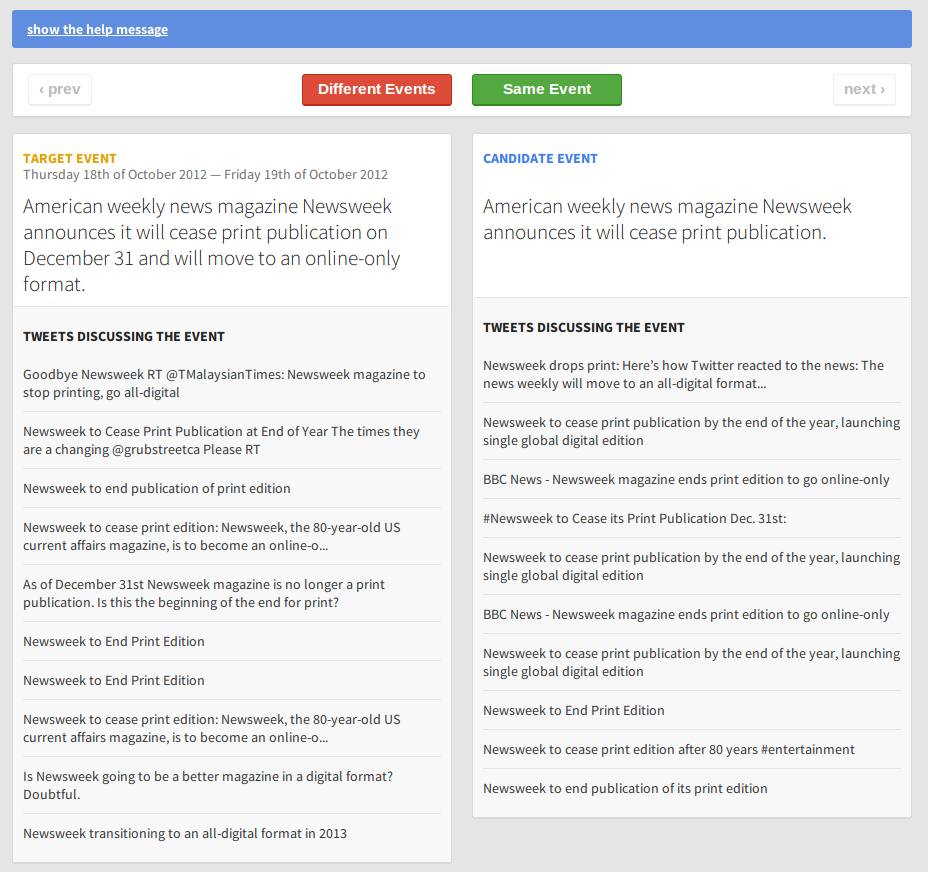
\includegraphics[width=\textwidth]{./Chapters/Collection/images/cluster_eval}}
	\caption{A screenshot of the cluster quality evaluation interface used by Mechanical Turk workers}
	\label{fig:clusteringscreenshot}
\end{figure}